\section{Andmestiku loomine}
Selles peatükis käsitletakse andmestiku loomise protsessi, sealhulgas andmete kogumist, töötlemist ja maskimist. Andmestiku loomine on oluline samm igasuguste andmete analüüsimisel ja seda ka masinõppe projektide puhul. Andmete kvaliteet ja sobivus mõjutavad otseselt mudeli täpsust ja usaldusväärsust. Nagu muudes valdkondades kehtib ka informaatikas Pareto printsiip, mille kohaselt 80\% probleemidest tuleneb 20\% põhjustest. Seega on andmestiku loomine ja töötlemine äärmiselt oluline etapp, mis võib määrata kogu projekti edasise käigu.

\subsection{Raie piirkonna andmete kogumine}
Metsateatis on dokument, mille kaudu metsaomanik esitab Keskkonnaametile
kavandatavate raietööde või oluliste metsakahjustuste kohta teabe. Keskkonnaamet
kontrollib esitatud teatiste nõuetekohasust ning veendub, et kavandatav raie
vastab kehtivatele õigusaktidele. Metsateatised menetletakse ja säilitatakse
riiklikus metsaregistris. Peale edukat menetlemist võib raietöödega alustada 10 päeva peale otsust ja kuni 24 kuu jooksul. \cite{MetsateatisJaMetsaregister} Metsateatised on avalikud ja neid saab vaadata riiklikus metsaregistris.

Koostöös Keskkonnaametiga (envir) saadi andmed metsateatistest, mis sisaldavad teavet nii metsateatise esitamise kuupäeva, metsateatise menetlemise kuupäeva, metsateatise kehtivuse alguskuupäeva kui ka metsateatise kehtivuse lõppkuupäeva kohta. Kuna riigimetsade teatised on täpsemas seisukorras, siis võeti need raieteatised selle uurimustöö aluseks. Seoses sellega et ühe lõigu peal võib olla väga väike kogus metsa, sai teatiste pärimine ümber ehitatud sedasi, et ühe metsa raie ümber kogutakse peale raie toimumist kokku ka kõik teised piirkonnad, millel on teada kas on mets või raieala. Piirkonniti pärimine sai teostatud kasutades PostGISi liidestust Postgresi andmebaasiga. Iga raie sisaldab ka endas geomeetria veergu, mis esitab polügooni kujul selle asukohta.

% TODO: eelnevas lõigus teha arusaadavamaks, mis on lõik millest räägitakse, eelnevalt juttu kuupäevadest jm teabest ja siis võib jääda segaseks. lisaks palun täpsustada: kogutakse kokku ka teised ... raadiuses asuvad piirkonnad

\begin{figure}[hb]
    \centering
    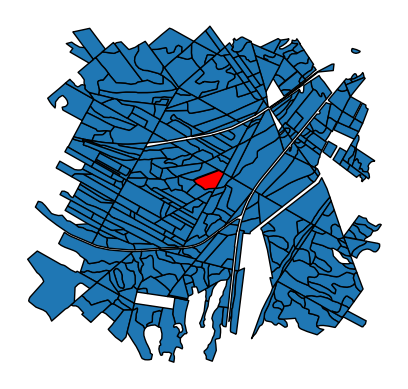
\includegraphics[width=.5\textwidth]{figures/andmestik/er_id_is10124223.png}
    \caption{Näidis ühe lageraie päringust saadud ümbrus}
    \label{fig:umbrusexample}
\end{figure}

Polügoon on geomeetriline kujund, mis määratleb kindla ala, ühendades üksteisega
punktid, et moodustada suletud piirjoon. Andmetöötluse ja ruumiandmete analüüsi
kontekstis kasutatakse polügoone, et täpselt määratleda geograafilisi alasid. \cite{WhatLocationPolygon}

See on terve andmetöötlus workflow!!!
\begin{figure}[H]
    \centering
    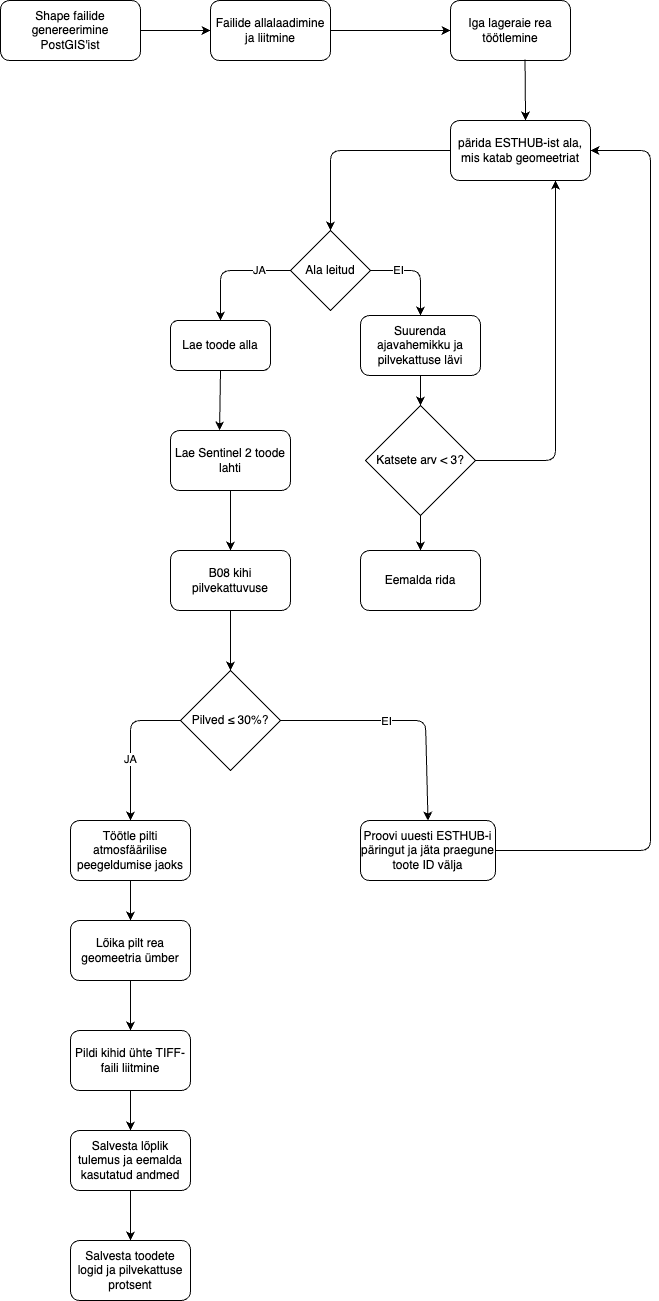
\includegraphics[width=.8\textwidth]{figures/andmestik/andmete_voog.drawio.png}
    \caption{Andmestiku loomise töövoog}
    \label{fig:terveflow}
\end{figure}

%\begin{itemize}
%    \item kust andmeid saab
%    \item kuidas andmeid töödelda
%    \begin{itemize}
%        \item kuidas andmeid puhastada
%        \item kuidas andmeid ühendada
%        \item kuidas andmeid lõigata
%        \item kuidas andmeid venitada
%        \item kui andmeid on puudu või kuidas filtreerida
%    \end{itemize}
%    \item kuidas andmeid maskida
%\end{itemize}
